\documentclass[border=6pt]{standalone}
\usepackage{amsmath}
\usepackage{amssymb}
\usepackage{tikz}
\usepackage{pgfplots}
\pgfplotsset{compat=1.18}
\usetikzlibrary{arrows.meta,calc,positioning}
\begin{document}
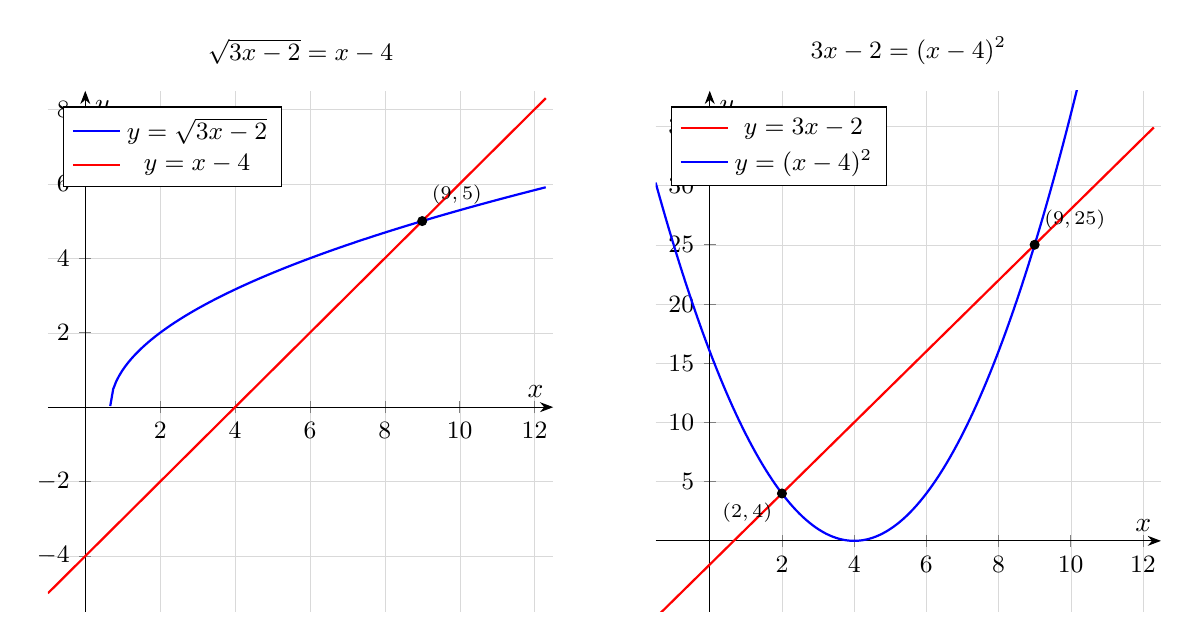
\begin{tikzpicture}
\begin{axis}[name=ax1,
    axis lines = middle,
    xlabel = {$x$}, ylabel = {$y$},
    grid=both,
    grid style={line width=.1pt, draw=gray!30},
    axis line style={-Stealth},
    legend style={font=\small},
    tick label style={font=\small},
    xmin=-1, xmax=12.5, ymin=-5.5, ymax=8.5,
    xtick={0,2,4,6,8,10,12},
    ytick={-4,-2,0,2,4,6,8},
    width=8cm, height=8.2cm,
    title={\small $\sqrt{3x-2}=x-4$},
    legend pos=north west,
]
\addplot[domain=0.667:12.3, samples=150, thick, blue] {sqrt(3*x-2)};
\addlegendentry{$y=\sqrt{3x-2}$}
\addplot[domain=-1:12.3, samples=2, thick, red] {x-4};
\addlegendentry{$y=x-4$}
\addplot[only marks, mark=*, mark size=1.6pt, black] coordinates {(9,5)};
\node[anchor=south west, font=\scriptsize] at (axis cs:9,5.2) {$(9,5)$};
\end{axis}
\begin{axis}[at={(ax1.south east)}, anchor=south west, xshift=1.3cm,
    axis lines = middle,
    xlabel = {$x$}, ylabel = {$y$},
    grid=both,
    grid style={line width=.1pt, draw=gray!30},
    axis line style={-Stealth},
    legend style={font=\small},
    tick label style={font=\small},
    xmin=-1.5, xmax=12.5, ymin=-6, ymax=38,
    xtick={0,2,4,6,8,10,12},
    ytick={0,5,10,15,20,25,30,35},
    width=8cm, height=8.2cm,
    title={\small $3x-2=(x-4)^2$},
    legend pos=north west,
]
\addplot[domain=-1.5:12.3, samples=2, thick, red] {3*x-2};
\addlegendentry{$y=3x-2$}
\addplot[domain=-1.5:12.3, samples=150, thick, blue] {(x-4)^2};
\addlegendentry{$y=(x-4)^2$}
\addplot[only marks, mark=*, mark size=1.6pt, black] coordinates {(2,4) (9,25)};
\node[anchor=north east, font=\scriptsize] at (axis cs:2,4) {$(2,4)$};
\node[anchor=south west, font=\scriptsize] at (axis cs:9,25.5) {$(9,25)$};
\end{axis}
\end{tikzpicture}
\end{document}
